\documentclass[11pt]{article}

\usepackage{CMPSC465}
\usepackage{enumitem}
\usepackage{algpseudocode}
\usepackage{tikz}
\usepackage{amsmath}
\usepackage{tikz} 
\usepackage{graphicx}
\usepackage[colorlinks=true, allcolors=blue]{hyperref}
\usepackage{tkz-graph}
\PassOptionsToPackage{usenames,dvipsnames,svgnames}{xcolor}  
\usepackage{tikz}
\usetikzlibrary{arrows,positioning,automata}
\def\title{Solution 05}

\def\defeq{\mathrel{\mathop:}=}
%\usepackage{algpseudocode}
%\usepackage{algorithm}
%\usepackage[ruled]{algorithm2e}
%\usepackage{amsthm}


\def\defeq{\mathrel{\mathop:}=}
%\usepackage{algpseudocode}
%\usepackage{algorithm}
\usepackage[ruled,noline]{algorithm2e}
%\usepackage{amsthm}
\newcommand\nonl{%
  \renewcommand{\nl}{\let\nl\oldnl}}% Remove line number for one line
  
\newcommand{\aaa}[1]{\hspace{0.65cm}\parbox[t]{15.3cm}{#1}}
\newcommand{\aab}[1]{\hspace{1.15cm}\parbox[t]{15.0cm}{#1}}
\newcommand{\aac}[1]{\hspace{1.65cm}\parbox[t]{15.0cm}{#1}}
\newcommand{\aad}[1]{\hspace{2.15cm}\parbox[t]{15.0cm}{#1}}
\newcommand{\aaA}[2]{\hspace{0.5cm} {\tikz[overlay] \draw (0.1, -0.1) -- (0.1, #1 * -1.5em + 0.6em);} \parbox[t]{15.0cm}{#2}}
\newcommand{\aaB}[2]{\hspace{1.0cm} {\tikz[overlay] \draw (0.1, -0.1) -- (0.1, #1 * -1.5em + 0.6em);} \parbox[t]{15.0cm}{#2}}
\newcommand{\aaC}[2]{\hspace{1.5cm} {\tikz[overlay] \draw (0.1, -0.1) -- (0.1, #1 * -1.5em + 0.6em);} \parbox[t]{15.0cm}{#2}}
\newcommand{\aaD}[2]{\hspace{2.0cm} {\tikz[overlay] \draw (0.1, -0.1) -- (0.1, #1 * -1.5em + 0.6em);} \parbox[t]{15.0cm}{#2}}
\newcommand{\xxx}{\par\vspace{0.1cm}}
\usepackage{tikz}

\begin{document}
\maketitle



\begin{qunlist}

% Manohar
\q{10}{}
Consider the following directed graph.
\\\\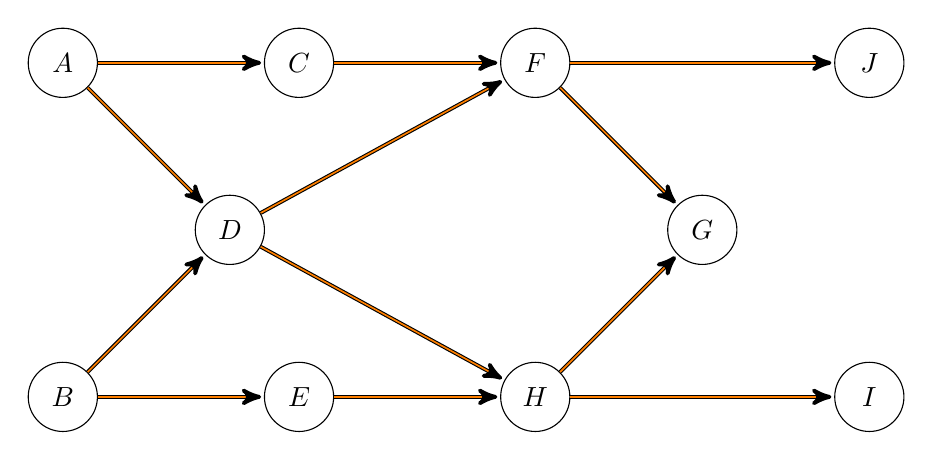
\begin{tikzpicture}[>=stealth',shorten >=1pt,node distance=3cm,on grid,initial/.style    ={}][!hb]
  \node[state]          (A)                        {$A$};
  \node[state]          (C) [right =of A]    {$C$};
  \node[state]          (D) [below right =of A]    {$D$};
  \node[state]          (B) [below left =of D]          {$B$};
  \node[state]          (E) [ right =of B]    {$E$};
  \node[state]          (F) [right =of C]    {$F$};
  \node[state]          (G) [below right =of F]    {$G$};
  \node[state]          (H) [right =of E]    {$H$};
  \node[state]          (I) [below right =of G]    {$I$};
  \node[state]          (J) [above right =of G]    {$J$};

\tikzset{mystyle/.style={->,double=orange}} 
\tikzset{every node/.style={fill=white}} 
\path (A)     edge [mystyle] (C)
      (A)     edge [mystyle] (D) 
      (B)     edge [mystyle] (E)
      (B)     edge [mystyle] (D)
      (C)     edge [mystyle] (F)
      (D)     edge [mystyle] (F)
      (D)     edge [mystyle] (H)
      (E)     edge [mystyle] (H)
      (H)     edge [mystyle] (G)
      (F)     edge [mystyle] (G)
      (F)     edge [mystyle] (J)
      (H)     edge [mystyle] (I); 
\end{tikzpicture}
\begin{enumerate}
    \item  What are the sources and sinks of the graph?
    \item  Give one linearization of this graph.
    \item  How many linearization does this graph have?
\end{enumerate}

\textbf{Solution:} 
\begin{enumerate}
    \item Sources of a graph do not have any in-edges. So, $A$ and $B$ are the sources. Sinks do not have any out-edges. So $J$, $G$ and $I$ are the sinks.
    \item $(A, B, C, D, E, F, H, G, I, J)$ is one of linearizations. 
    \item It has 356 linearizations. Consider $F$ and $H$; first assume that $F$ is before $H$ in the linearization. What are the possible situations between $F$ and $H$ in the linearization? There are 5 cases:
        \begin{enumerate}
        \item $FH$. Then ${A,B,C,D,E}$ are before it and $G,J,I$ are after it. 
        It is not hard to calculate that the number of linearizations for the former is 16 and the number of linearization for the latter is 6.
        \item $FEH$. Then ${A,B,C,D}$ are before it and $G,J,I$ are after it. 
        The number of linearizations for the former is 5 and the number of linearization for the latter is 6.
        \item $FJH$. Then ${A,B,C,D,E}$ are before it and $G,I$ are after it. The number of linearizations for the former is 16 and the number of linearization for the latter is 2.
        \item $FEJH$. Then ${A,B,C,D}$ are before it and $G,I$ are after it. The number of linearizations for the former is 5 and the number of linearization for the latter is 2.
        \item $FJEH$. Then ${A,B,C,D}$ are before it and $G,I$ are after it. The number of linearizations for the former is 5 and the number of linearization for the latter is 2.
        \end{enumerate}
        Summing them up gives $16\cdot 6 + 5 \cdot 6 + 16 \cdot 2 + 5 \cdot 2 + 5 \cdot 2 = 178$. Don't forget this is under the assumption that $F$ is before $H$, the other way around is symmetric. So the total number of linearization is $178\cdot 2 = 356$.
    
\end{enumerate}


% Manohar
\q{10}{} Consider the following directed graph.
\\\\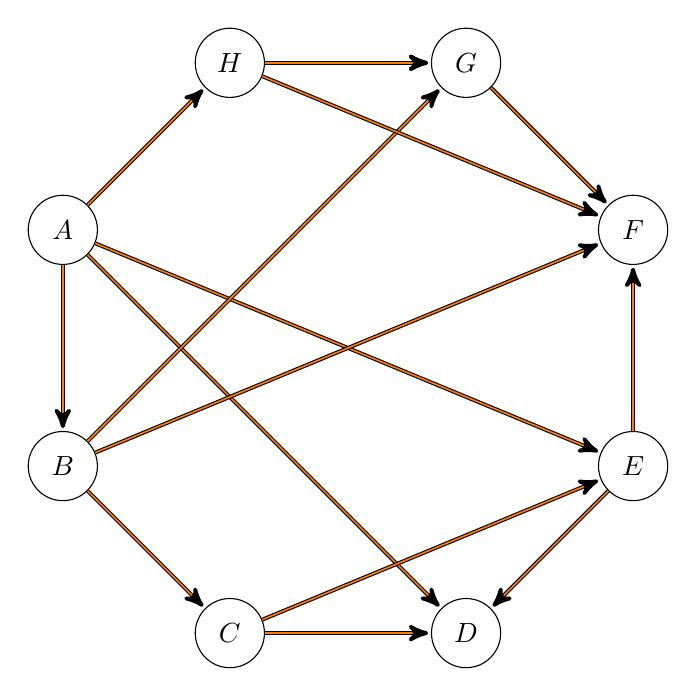
\begin{tikzpicture}[>=stealth',shorten >=1pt,node distance=3cm,on grid,initial/.style    ={}][!hb]
  \node[state]          (A)                        {$A$};
  \node[state]          (B) [below =of A]    {$B$};
  \node[state]          (C) [below right =of B]    {$C$};
  \node[state]          (D) [right =of C]          {$D$};
  \node[state]          (E) [above right =of D]    {$E$};
  \node[state]          (F) [above =of E]    {$F$};
  \node[state]          (G) [above left =of F]    {$G$};
  \node[state]          (H) [left =of G]    {$H$};

\tikzset{mystyle/.style={->,double=orange}} 
\tikzset{every node/.style={fill=white}} 
\path (A)     edge [mystyle] (B)
      (A)     edge [mystyle] (D) 
      (A)     edge [mystyle] (E)
      (B)     edge [mystyle] (C)
      (B)     edge [mystyle] (G)
      (B)     edge [mystyle] (F)
      (C)     edge [mystyle] (E)
      (C)     edge [mystyle] (D)
      (E)     edge [mystyle] (D)
      (E)     edge [mystyle] (F)
      (H)     edge [mystyle] (F)
      (H)     edge [mystyle] (G)
      (G)     edge [mystyle] (F)
      (H)     edge [mystyle] (G)
      (A)     edge [mystyle] (H); 
\end{tikzpicture}

\begin{enumerate}
    \item  Perform depth-first search with timing (DFS-with-timing) on the above graph; whenever there’s a choice of vertices, pick the one that is alphabetically first: give the pre and post number of each vertex.
    \item  Draw the meta-graph of this graph, and give the vertices in each connected component.
\end{enumerate}


\textbf{Solution:} 


\begin{enumerate}
    \item  A: 1,16\\
           B: 2,13\\
           C: 3,10\\
           D: 4,5\\
           E: 6,9\\
           F: 7,8\\
           G: 11,12\\
           H: 14,15
    \item  As there are no cycles in the graph, meta graph of the given graph is itself.
\end{enumerate}

% Manohar
\q{10}{}
You are in charge of the United States Mint. The money-printing machine has developed a strange bug: it will only print a bill if you give it one first. If you give it a d-dollar bill, it is only willing to print bills of
value $d^2 \mod 400$ and $d^2 +1 \mod 400$. For example, if you give it a \$6 bill, it is willing to print \$36 and
\$37 bills, and if you then give it a \$36-dollar bill, it is willing to print  \$96 and \$97. %(1296 (mod 400) = 96.)

You start out with only a \$1 bill to give the machine. Every time the machine prints a bill, you are allowed to give that bill back to the machine, and it will print new bills according to the rule described above. You
want to know if there is a sequence of actions that will allow you to print a \$20 bill, starting from your \$1 bill. Model this task as a graph problem: give a precise definition of the graph (what are the vertices and edges) involved and state the specific question about this graph that needs to be answered. Give an algorithm to solve the stated problem and give the running time of your algorithm.

\textbf{Solution:} 
$G = (V, E)$.

$V$: we have at most 400 possible bills (includes \$0 bill). We add 400 vertices $V = \{v_1, v_2, ..., v_{400}\}$ to represent these 400 possible bills (e.g. $v_1$ represents \$1 bill, $v_5$ represents \$5 bill, and $v_{400}$ represent \$0 bill which can be generated by giving \$20). 

$E$: we enumerate all vertices to add edges. For each vertices $v_k$, we have $i = k^2 \mod 400$ and $j = k^2 +1 \mod 400$, so we add a directed edge from $v_k$ to $v_i$ and a directed edge from $v_k$ to $v_j$.

Then the problem becomes if there is a path to reach $v_{20}$ from a given vertex $v_1$ in the built graph $G$.

We can apply the \emph{explore} algorithm start from $v_1$ to solve this problem. The running time for applying \emph{explore} algorithm is $O(|V|+|E|)$. The running time for creating vertices and edges is $O(|V|+|E|)$. So the total running time is $O(|V|+|E|)$.

\newpage
{\huge {\bf Rubrics:}}

\bigskip


{\bf Problem 1, 10pts}
\begin{itemize}
    \item 2 points : Provided the correct answer.
    \item 3 points : Provided a correct linearization.
    \item 5 points(Bonus) : Provided the correct answer.
    \item 1 point: I don't know how to answer this question
\end{itemize}
{\bf Problem 2, 10pts}
\begin{itemize}
    \item 6 points : Provided the correct pre an post numbers for all nodes.
    \item 3 points : Provided a correct pre and post number but didn't follow alphabetical order when there is a choice of vertices.
    \item 4 points : identified that metagraph is the given graph itself.(no need to draw the graph).
    \item 1 point: I don't know how to answer this question
\end{itemize}

{\bf Problem 3, 10pts}
\begin{itemize}
    \item 5 points: construct the graph correctly
    \begin{itemize}
        \item 2 points : add vertices correctly
        \item 3 points : add edges correctly
    \end{itemize}

    \item 5 points: correct algorithm and running time analysis
    \begin{itemize}
        \item 1 points : transfer the problem correctly (e.g. check if there is a path from $v_1$ to $v_{20}$)
        \item 3 points : apply explore algorithm
        \item 1 points : appropriate running time analysis
    \end{itemize}
    
    \item 1 point: I don't know how to answer this question
\end{itemize}

\end{qunlist}
\end{document}
